\documentclass{article}
\usepackage[utf8]{inputenc}
\usepackage{amsthm}
\usepackage{natbib}
\usepackage{graphicx}
\usepackage{tikz}
\usetikzlibrary{arrows}

% COMMANDS
\newcommand{\basis}{\newline \noindent {\bf Basis:} }
\newcommand{\ih}{\newline \noindent {\bf Induction hypothesis:}  Assume }
\newcommand{\is}{\newline \noindent {\bf Induction:} }


\begin{document}

\newtheorem*{thm}{Theorem}

\begin{thm}
For every $t\ge3$, there existsa graph $G_t$ so that
$\chi(G_t)=t$ and $\omega(G_t)=2$.
\end{thm}

\begin{proof}
By induction on $n$, the number of people.
\basis
For $t=3$, consider the cycle $C_5$:\\

\begin{center}
    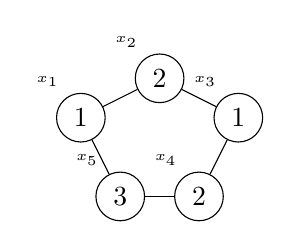
\begin{tikzpicture}[auto,node distance=3cm,
        main node/.style={circle,draw}]
      
        \node[main node] [label=120:\tiny{$x_1$}] (1) at (0,0) {1};
        \node[main node] [label=120:\tiny{$x_2$}] (2) at (1,.5) {2};
        \node[main node] [label=120:\tiny{$x_3$}] (3) at (2,0) {1};
        \node[main node] [label=120:\tiny{$x_4$}] (4) at (1.5,-1) {2};
        \node[main node] [label=120:\tiny{$x_5$}] (5) at (.5,-1) {3};
      
        \path[every node/.style={font=\sffamily\small}]
          (1) edge node {} (2)
          (2) edge node {} (3)
          (3) edge node {} (4)
          (4) edge node {} (5)
          (5) edge node {} (1);
      \end{tikzpicture}\\
\end{center}

Which can also be drawn as:\\

\begin{center}
    \begin{tikzpicture}[auto,node distance=1cm,
        main node/.style={circle,draw}]
      
        \node[main node] [label=120:\tiny{$x_1$}] {1};
        \node[main node] [label=120:\tiny{$x_2$}] (2) [right of=1] {2};
        \node[main node] [label=120:\tiny{$x_3$}] (3) [right of=2] {1};
        \node[main node] [label=120:\tiny{$x_4$}] (4) [right of=3] {2};
        \node[main node] [label=120:\tiny{$x_5$}] (5) [right of=4] {3};
      
        \path[every node/.style={font=\sffamily\small}]
          (1) edge node {} (2)
          (2) edge node {} (3)
          (3) edge node {} (4)
          (4) edge node {} (5)
          (5) edge [bend left] node {} (1);
      \end{tikzpicture}\\
\end{center}

As we see, $\chi(G_3)=3$ and $\omega(G_3)=2$.\\
\ih
\is
Assume that for $t\ge3$, we have determined the graph $G_t$.
Suppose that $G_t$ has $n_t$ vertices. Lebel the vertices
$x_1, x_2, x_3, \dots, x_{n_t}$.\\

\begin{center}
    \begin{tikzpicture}[auto,node distance=1cm,
        minimum size=.5cm,
        main node/.style={circle,draw}]
      
        \node[main node] [label=120:\tiny{$x_1$}] {};
        \node[main node] [label=120:\tiny{$x_2$}] (2) [right of=1] {};
        \node[main node] [label=120:\tiny{$x_3$}] (3) [right of=2] {};
        \node[main node] [dashed] (4) [right of=3] {};
        \node[main node] [dashed] (5) [right of=4] {};
        \node[main node] [label=120:\tiny{$x_{n_t}$}] (n) [right of=5] {};
      
        \path[every node/.style={font=\sffamily\small}]
          (1) edge node {} (2)
          (2) edge node {} (3)
          (3) edge [dashed] node {} (4)
          (4) edge [dashed] node {} (5)
          (5) edge [dashed] node {} (n)
          (n) edge [bend left] node {} (1);
      \end{tikzpicture}\\
\end{center}

To construct $G_{t+1}$ we begin by copying the vertices, 
from $G_t$ (no edges) into an independent set
and calling it $ I = \{y_1, y_2, y_3, \dots, y_{n_t}\} $.\\

\begin{center}
    \begin{tikzpicture}[auto,node distance=1cm,
        minimum size=.5cm,
        main node/.style={circle,draw}]
      
        \node[main node] [label=\tiny{$y_1$}] {};
        \node[main node] [label=\tiny{$y_2$}] (2) [right of=1] {};
        \node[main node] [label=\tiny{$y_3$}] (3) [right of=2] {};
        \node[main node] [dashed] (4) [right of=3] {};
        \node[main node] [dashed] (5) [right of=4] {};
        \node[main node] [label=\tiny{$y_{n_t}$}] (n) [right of=5] {};
      \end{tikzpicture}\\
\end{center}

We then add a copy $H_t$ of $G_t$ with $y_i$ adjacent to $x_j$
if and only if $x_i$ is adjacent to $x_j$. In other words
\\

\begin{center}
    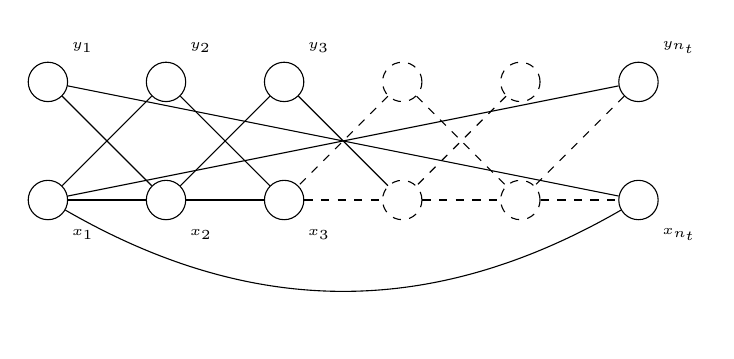
\begin{tikzpicture}[auto,node distance=1.5cm,
        minimum size=.5cm,
        main node/.style={circle,draw}]
      
        \node[main node] [label={above right:\tiny{$y_1$}}] (y1) {};
        \node[main node] [label={above right:\tiny{$y_2$}}] (y2) [right of=y1] {};
        \node[main node] [label={above right:\tiny{$y_3$}}] (y3) [right of=y2] {};
        \node[main node] [dashed] (y4) [right of=y3] {};
        \node[main node] [dashed] (y5) [right of=y4] {};
        \node[main node] [label={above right:\tiny{$y_{n_t}$}}] (yn) [right of=y5] {};
        \node[main node] [label={below right:\tiny{$x_1$}}] (x1) [below of=y1] {};
        \node[main node] [label={below right:\tiny{$x_2$}}] (x2) [right of=x1] {};
        \node[main node] [label={below right:\tiny{$x_3$}}] (x3) [right of=x2] {};
        \node[main node] [dashed] (x4) [right of=x3] {};
        \node[main node] [dashed] (x5) [right of=x4] {};
        \node[main node] [label={below right:\tiny{$x_{n_t}$}}] (xn) [right of=x5] {};
      
        \path[every node/.style={font=\sffamily\small}]
          (x1) edge node {} (x2)
          (x2) edge node {} (x3)
          (x3) edge [dashed] node {} (x4)
          (x4) edge [dashed] node {} (x5)
          (x5) edge [dashed] node {} (xn)
          (xn) edge [bend left] node {} (x1)
          (y1) edge node {} (x2)
          (y1) edge node {} (xn)
          (y2) edge node {} (x1)
          (y2) edge node {} (x3)
          (y3) edge node {} (x2)
          (y3) edge node {} (x4)
          (y4) edge [dashed] node {} (x3)
          (y4) edge [dashed] node {} (x5)
          (y5) edge [dashed] node {} (x4)
          (yn) edge [dashed] node {} (x5)
          (yn) edge node {} (x1)
          ;
    \end{tikzpicture}\\
\end{center}

Finally we attach a new vertex $z$ adjacent to all vertices in $I$\\

\begin{center}
    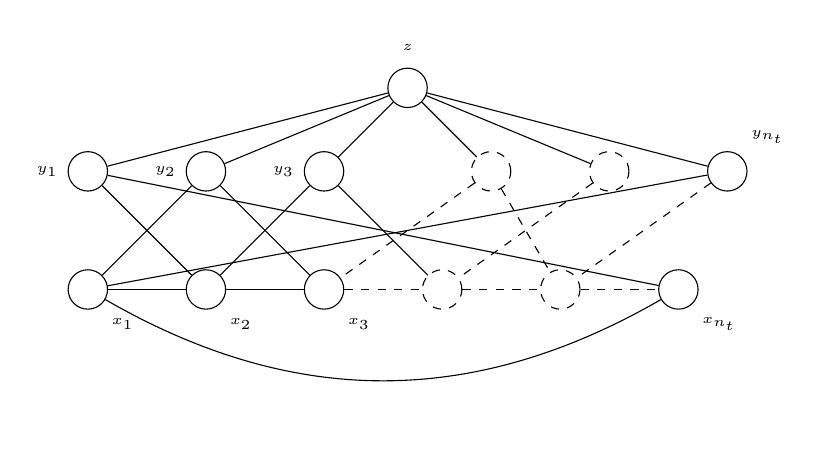
\begin{tikzpicture}[auto,node distance=1.5cm,
        minimum size=.5cm,
        main node/.style={circle,draw}]
    
        \node[main node] [label={above:\tiny{$z$}}] (z) {};
        \node[main node] [label={left:\tiny{$y_3$}}] (y3) [below left of=z] {};
        \node[main node] [label={left:\tiny{$y_2$}}] (y2) [left of=y3] {};
        \node[main node] [label={left:\tiny{$y_1$}}] (y1) [left of=y2] {};
        \node[main node] [dashed] (y4) [below right of=z] {};
        \node[main node] [dashed] (y5) [right of=y4] {};
        \node[main node] [label={above right:\tiny{$y_{n_t}$}}] (yn) [right of=y5] {};
        \node[main node] [label={below right:\tiny{$x_1$}}] (x1) [below of=y1] {};
        \node[main node] [label={below right:\tiny{$x_2$}}] (x2) [right of=x1] {};
        \node[main node] [label={below right:\tiny{$x_3$}}] (x3) [right of=x2] {};
        \node[main node] [dashed] (x4) [right of=x3] {};
        \node[main node] [dashed] (x5) [right of=x4] {};
        \node[main node] [label={below right:\tiny{$x_{n_t}$}}] (xn) [right of=x5] {};
    
        \path[every node/.style={font=\sffamily\small}]
        (x1) edge node {} (x2)
        (x2) edge node {} (x3)
        (x3) edge [dashed] node {} (x4)
        (x4) edge [dashed] node {} (x5)
        (x5) edge [dashed] node {} (xn)
        (xn) edge [bend left] node {} (x1)
        (y1) edge node {} (x2)
        (y1) edge node {} (xn)
        (y2) edge node {} (x1)
        (y2) edge node {} (x3)
        (y3) edge node {} (x2)
        (y3) edge node {} (x4)
        (y4) edge [dashed] node {} (x3)
        (y4) edge [dashed] node {} (x5)
        (y5) edge [dashed] node {} (x4)
        (yn) edge [dashed] node {} (x5)
        (yn) edge node {} (x1)
        (z) edge node {} (y1)
        (z) edge node {} (y2)
        (z) edge node {} (y3)
        (z) edge node {} (y4)
        (z) edge node {} (y5)
        (z) edge node {} (yn)
        ;
    \end{tikzpicture}\\
\end{center}

Now to determine $\omega(G_{t+1})$ let's look at the cases
that there might be a triangle ($C_3$) present in $G_{t+1}$:\\

\textbf{\textit{Case I}}
    The traingle comprises of $z$ and 2 nodes from $I$:\\
    This case is \textbf{not possible} 
    since the nodes in $I$ are not adjacent to each other.

\textbf{\textit{Case II}}
    The traingle comprises of 3 nodes from $I$:\\
    This case is \textbf{not possible} 
    since the nodes in $I$ are not adjacent to each other.

\textbf{\textit{Case III}}
    The traingle comprises of 3 nodes from $H_t$:\\
    This case is \textbf{not possible} 
    since there is no triangle in $H_t$
    ($\omega(H_t) = \omega(G_t) = 2$,
    from the premise).

\textbf{\textit{Case IV}}
    The traingle comprises of $z$, a node from $I$
    and another, from $H_t$:\\
    This case is \textbf{not possible} 
    since $z$ is is not adjacent to any node in $H_t$.\\

\textbf{\textit{Case V}}
    The traingle comprises of $z$, a 2 nodes
    from $H_t$:\\
    This case is \textbf{not possible} 
    since $z$ is is not adjacent to any node in $H_t$.\\

\textbf{\textit{Case VI}}
    The traingle comprises of one node
    from $H_t$ and 2 nodes 
    from $I$:\\
    This case is \textbf{not possible} 
    since the nodes in $I$ are not adjacent to each other.

\textbf{\textit{Case VII}}
    The traingle comprises of one node
    from $I$ and 2 nodes
    from $H_t$:\\
    This case is \textbf{not possible} 
    since every node in $I$ is adjacent To
    exactly 2 nodes in $H_t$ that are not adjacent.

Therefore, $\omega(G_{t+1})=2$

\end{proof}

\bibliographystyle{plain}
\bibliography{references}
\end{document}